\makeatletter                                                   
\def\input@path{{../}}                                          
\makeatother                                                    
\documentclass[../main.tex]{subfiles}                           
\begin{document}                                                
\chapter{A 4th party logistics optimizer}
\label{ch:appr}
This chapter explains how we build our model, the fourth party logistics optimizer (4PLO).
The first section \cref{sec:alns}, desribes the meta heuristic approach 
The first \cref{sec:init} explain how we have chosen the initial solution.\par
Then \cref{sec:heur} present each of the heuristics included in the basic version of our model.
The next \cref{sec:choos}, explains how our model is choosing a heuristic in a given iteration. 
Then \cref{sec:weight} explain how our algorithm is using the performance history of heuristics to adapt the weights of the heuristics 

\Cref{sec:wild} present the wild escape algorithm used to prevent that our model gets stuck in a local optimum.

\section{ALNS for 4th party logistic problems}
\label{sec:alns}
Our metaheuristic is similar to the ALNS approach introduced by \cite{ropke06}, but we have adapted it to specifically solve our fourth party logistics problem. 
Our approach will be explained over the next few sections but the ALNS implementation differs mainly in the following way:
\begin{enumerate}
    \item Our heuristics each contain one removal and one insertion heuristic and are not chosen separately. 
    \item We integrate an escape algorithm to avoid that the algorithm gets stuck.
\end{enumerate}

A brief pseudocode of our implementation of ALNS for 4th party logistic problems is described in \cref{alg:alns}.  

\begin{algorithm}
    \caption{ALNS for 4th party logistic problems}\label{alg:alns}
    \begin{algorithmic}[1]
        \Function{alns}{}
        \State solution $s = generateInitialSolution()$
        \State solution $s_{best} = s$
        \State iterations since best solution found $i=0$
        \Repeat
            \If {$i>escape\ condition$}
                \State $s = wildEscape(s)$ 
            \EndIf
            \State $s' = s$
            \State select a heuristic, h, based on selection parameters
            \State $s' = applyHeuristic(h,s')$
            \If {$f(s') < f(s_{best})$}
                \State $s_{best}=s'$
            \EndIf
            \If {$accept(s', s)$}
                \State $s = s'$
            \EndIf
            \State update selection parameters and escape condition
        \Until {stop condition met}
        \State
        \Return $s_{best}$
        \EndFunction
    \end{algorithmic}
\end{algorithm}

The algorithm starts by picking an initial solution, and then moves into a loop where it picks a heuristic $h$, and an amount of orders $q$, before applying the heuristic to the current solution. 
It then updates the best solution and decides to accept the newly created solution or not until the stop condition is met.
At the start of the loop it checks if an escape condition is met where it will run \cref{alg:wild} on our current solution $s$. \par
We will now move on to explaining each step of the model more in detail.

\section{Initial Solution}
\label{sec:init}
Many different algorithms have been made for finding an initial solutions to a PDPTW. \cite{hosny12} found that the sequential construction sequence may be the most suitable construction algorithm for the MV-PDPTW. 
We have chosen to simply start with an initial solution where no orders are assigned to any vehicle, ie. all orders are assigned to the dummy vehicle in the solution permutation. 
We chose this because it is simple to implement, efficient in terms of running time and our model will be able to adapt to the problem on its own, regardless of the initial solution.

\section{Heuristics}
\label{sec:heur}
This section presents the heuristics used by our algorithm.
The first three heuristics7gc \ref{sec:swap}, \ref{sec:exch}, \ref{sec:2opt}, we call shuffeling heuristics. They try to quickly schuffle a given solution around to find new solutions in the same neighbourhood. \par

Removal and reinsertion heuristics are well reserached tools used in solving pickup and delivery problems. \cite{hemmati14} and \cite{hemmati16} use insertion and removal heuristics to solve benchmark tramp ship routing and scheduling problems and maritime shipping problems.
The last four heuristics, \ref{sec:rand}, \ref{sec:clust}, \ref{sec:greedy}, \ref{sec:shaw}, we refer to here as removal and reinsertion heuristics. Each of them contain one heuristic for removal and one heuristic for reinsertion.
These are used partly to move from one neighbourhood to another, and partly for local search depending on the amount of solution elements, $q$, being reinserted.  

\subsection{Swap}
\label{sec:swap}
This heuristic simply tries to swap the pickup and delivery of two different orders until the first time it finds a fit. 
\Cref{fig:swap} illustrates a successful swap between two orders in a simple solution permutation. 

\begin{figure}                                                                    
    \centering                                                                                     
    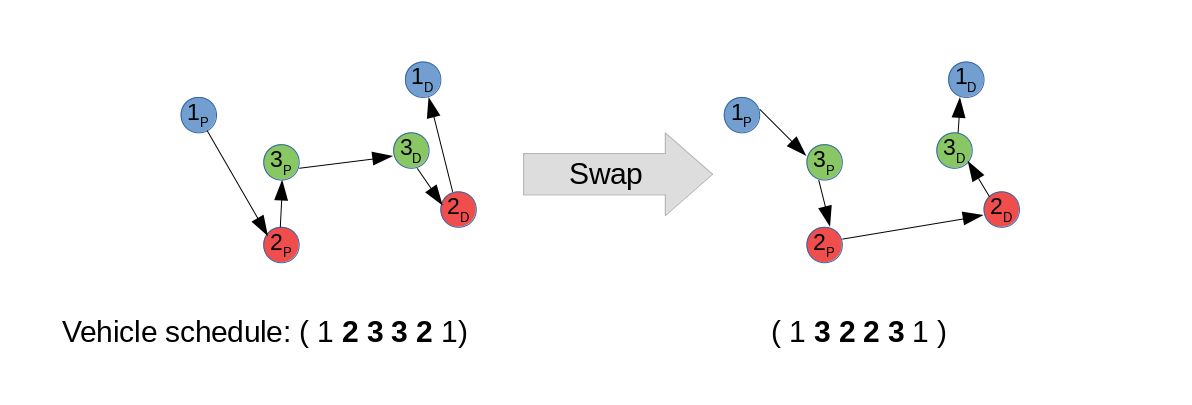
\includegraphics[width=\textwidth]{swap_ill}                                     
    \caption{A swap heuristic performed on a simple solution with two orders. The numbers indicate an order and the letters P and D indicate pickup and delivery respectively.}
    \label{fig:swap}
\end{figure}

This heuristic is very efficient and jumps randomly around a neighbourhoods solution space.

\subsection{3-exchange}
\label{sec:exch}
The 3-exchange heuristic selects a random vehicle with at least two assigned orders, and performs an exchange of 3 assigned positions until a feasible new combination is found. A 3-exchange of position 2, 4 and 6 in a simple permutation is illustrated by \cref{fig:exch}. \newline

\begin{figure}                                                                                     
    \centering                                                                                     
    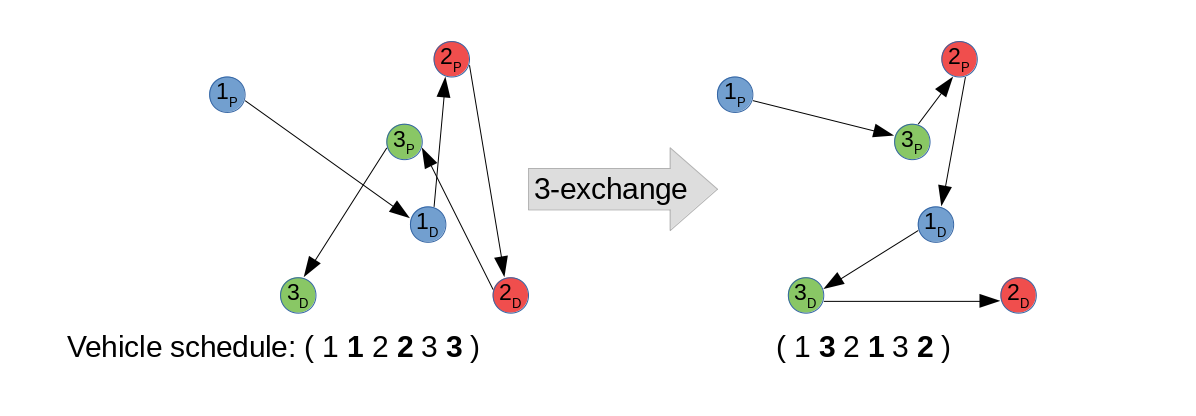
\includegraphics[width=\textwidth]{3-exchange_ill}                                     
    \caption{A 3-exchange heuristic performed on a simple solution with three orders. The numbers indicate an order and the letters P and D indicate pickup and delivery respectively.}
    \label{fig:exch}                                                                            
\end{figure}

This heuristic is very fast, as the exchanges are fast operations and checking if a vehicles schedule is feasible is also a very effective operation. Like the swap heuristic from the previous section this heuristic jumps randomly around a neighbourhoods solution space.

\subsection{2-opt}
\label{sec:2opt}
2-opt is a common heuristic used in travelling salesman problems aswell as with metaheuristics to solve VRP. \cite{lin65} implemented the 2-opt heuristic for travelling salesmen problem and \cite{bullnheimer99} combined 2-opt with the ant system metaheuristic.
The 2-opt heuristic used in this paper is similar to the heuristic from \cite{carrabs07}.
\Cref{fig:2opt} illustrates one iteration of our 2-opt heuristic on a simple permutation.

\begin{figure}                                                                                     
    \centering                                                                                 
    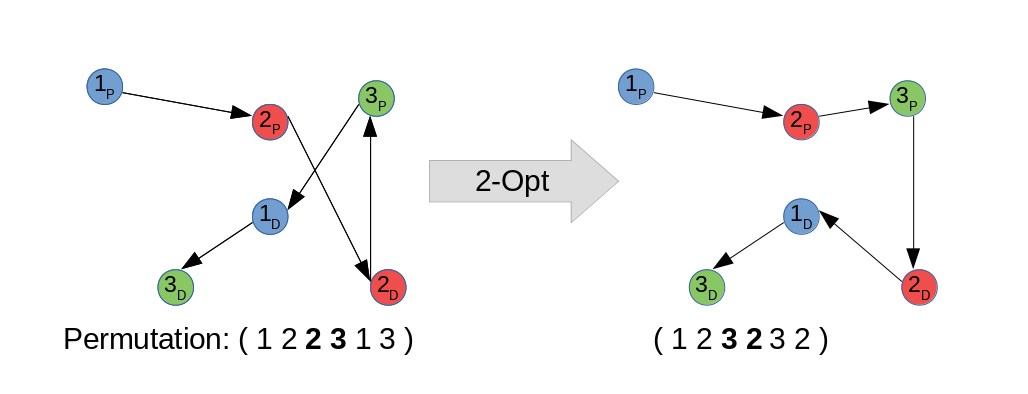
\includegraphics[width=\textwidth]{2-opt_ill}                                     
    \caption{One 2-opt heuristic operation performed on a simple solution with three orders. In this example $i=2$ and $j=4$ so the schedule $S_{ij}$ is reversed. The numbers indicate an order and the letters P and D indicate pickup and delivery respectively.}
    \label{fig:2opt}
\end{figure}

\begin{algorithm}
    \caption{2-opt heuristic}\label{alg:2opt}
    \begin{algorithmic}[1]
        \Function{twoOpt}{}
        \State select random vehicle $v$
        \State schedule $S = S_v$
        \Repeat
        \State $S_{best} = S$
        \For{$i<S.length$}
            \State $j=i+1$
            \For{$j<S.length$}
                \State schedule $ S' = S_{0i} + reverse(S_{(i+1)j}) + S_{(j+1)n}$ 
                \If {$f(S')<f(S_{best})$} 
                \State $S = S'$
                \EndIf
            \EndFor
        \EndFor
        \Until {no further improvement found}
        \State 
        \Return $S$
        \EndFunction
    \end{algorithmic}
\end{algorithm}


The heuristic is also described in \cref{alg:2opt} and it starts by selecting a random vehicle with more than 2 orders.
For the selected vehicle it divides up the schedule $S$ of the vehicle in 3 parts. 
All orders up until the index $i$ of the vehicle schedule are inserted normally. 
Orders from the index $j+1$ until the end of the schedule are also inserted normally. 
Then finally orders from the index i+1 until index j are inserted in reverse order.
If the new schedule has a smaller cost than the original schedule, the schedule is remembered as the new best route. 
When all reverses have been performed on the current route, the best route is selected as the new route.
This operation is continued until no improvement can be made ie. the best possible schedule for the selected vehicle has been found.

\subsection{Random fit}
\label{sec:rand}
In most problems there are solutions that you simply cannot find using pure logic. 
Constant minimizing costs and searching for the most efficient solution possible could lead you to always end up in the same local neighbourhoods, and not really exploring the whole solution space. 
We therefore decided to make one remove and reinsert heuristic that does not have any specific priorities but rather moves around neighbourhoods randomly. 

\begin{algorithm}
    \caption{Remove random and reinsert first fit heuristic}\label{alg:rand}
    \begin{algorithmic}[1]
        \Function{randomFit}{$s\in \{solution}$}
        \State select the number of orders to reinsert $q$
        \State solution $s' = s$
        \State remove $q$ orders from $s'$
        \State set I = removed orders
        \For{$z\in I$}
            \Repeat
            \State choose random vehicle $v$
            \State choose random position in schedule $S_v$
            \State insert $z$ in $S_v$
            \Until {feasible schedule found}
            \State update s'
        \EndFor
        \State
        \Return s'
        \EndFunction
    \end{algorithmic}
\end{algorithm}

\Cref{alg:rand} shows the pseudocode for our remove random insert first fit heuristic. 
It starts by selecting a random amount of orders $q$ which it is to remove and reinsert. 
Then it selects $q$ random orders and removes them from the solution. 


randomly between 2 orders and 10 percent of the amount of orders and reinserts them randomly in their first possible position. 
This heuristic is used to jump from one neighbourhood to another and is trying to search for possible solutions regardless of the cost they produce.

\subsection{Clustering}
\label{sec:clust}
\Cref{sec:4flow} illustrates how a typical 4PL customer typically have their factories and suppliers structured in clusters around a continent or a country. 
This led us to try to build a heuristic which considers clusters as a factor when removing and reinserting an order in a schedule. 
Orders delivered from and too different clusters by the same vehicle, should be removed. 
In the same way orders that are being delivered from and to similar clusters should be bundled together on vehicles. \par
To build a heuristic which takes advantage of this there challenges that needs to be overcome. 
How do we determine the size of our cluster? 
And after that how do we decide which locations belong in which cluster? 
The next two paragraphs will explain the methods we have used to solve this, before we go into detail on how our clustering heuristic is working.

\subsubsection{The siluette coefficient}
To decide which pickup and delivery locations belong to which clusters we first needed to find how many clusters we should have. 
In other words we need to find $k$, the amount of clusters best fitting to the problem. 
\cite{kaufman90} introduced an efficient way to compare clusters of different sizes by calculating the what they call a siluette coefficient.
The coefficient is calculated based on two aspects, cohesion $a_x$ and separation $b_x$ of a node (or in our case a location) $x$. 
Together these aspects make out the siluette $u$.
\begin{figure}
\centering
    \begin{subfigure}[b]{0.35\textwidth}
        \centering
        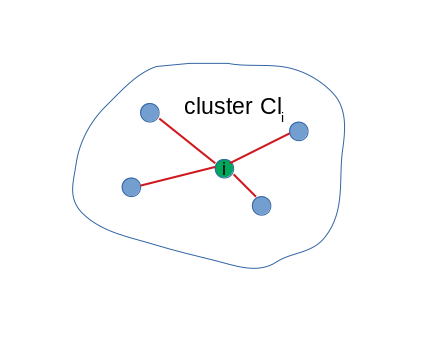
\includegraphics[width=\textwidth]{cohesion}
        \caption{Cohesion}
        \label{fig:cohesion}
    \end{subfigure}
    \hfill
    \begin{subfigure}[b]{0.60\textwidth}
        \centering
        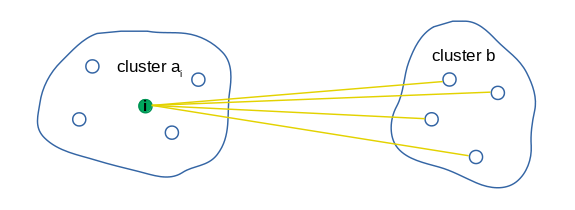
\includegraphics[width=\textwidth]{separation}
        \caption{Separation}
        \label{fig:separation}
    \end{subfigure}
    \label{fig:silu}
    \caption{The figures show the cohesion and separation effect illustrated respectively by the red and yellow lines. The green node represent location $i$ and $Cl_i$ is its cluster. The cluster $Cl_h$ is the cluster with the minimum average distance to $i$. }
\end{figure}


\Cref{fig:silu} illustrate the cohesion and sparation of a green node $i$ part of cluster $Cl_i$. 
The cohesion $a_i$ is the mean of the distance, $d_{ij}$, from $x$ to all other nodes in cluster $Cl_i$. The separation $b_i$ is the minimum of the mean of the distance to the nodes in all other clusters, which in the illustration is cluster B.
The two effects can be written as follows:
\begin{equation}
    \label{eq:cohesion}
    a_i = \dfrac{1}{|Cl_i|-1}\sum_{j\in Cl_i, i\neq j}{d_{ij}}
\end{equation}

\begin{equation}
    \label{eq:cohesion}
    b_i = \min_{h\neq i} \dfrac{1}{|Cl_h|}\sum_{i\neq j}{d_{ij}}
\end{equation}

The siluette coefficient $u_i$ for location $i$ is then calculated as follows: 

\begin{alignat} {2}
    \label{eq:siluette}
    a_i = \dfrac{b_i-a_i}{\max{a_i,b_i}}, &\quad\quad\quad\quad&& if\ |Cl_i|>1 \label{eq:siluette}\\
    a_i = 0,& && if\ |Cl_i| = 1 \nonumber
\end{alignat}

Comparing the siluette coefficient of one cluster to another requires that the nodes are divided into clusters. We will now explain how we found the best cluster for a given size $k$.

\subsubsection{Hirarchial single linkage clustering}
To find the best possible cluster of a given size $k$, we used something called hirarchial single linkage clustering algorithm.

\begin{figure}                                                                                     
    \centering                                                                                 
    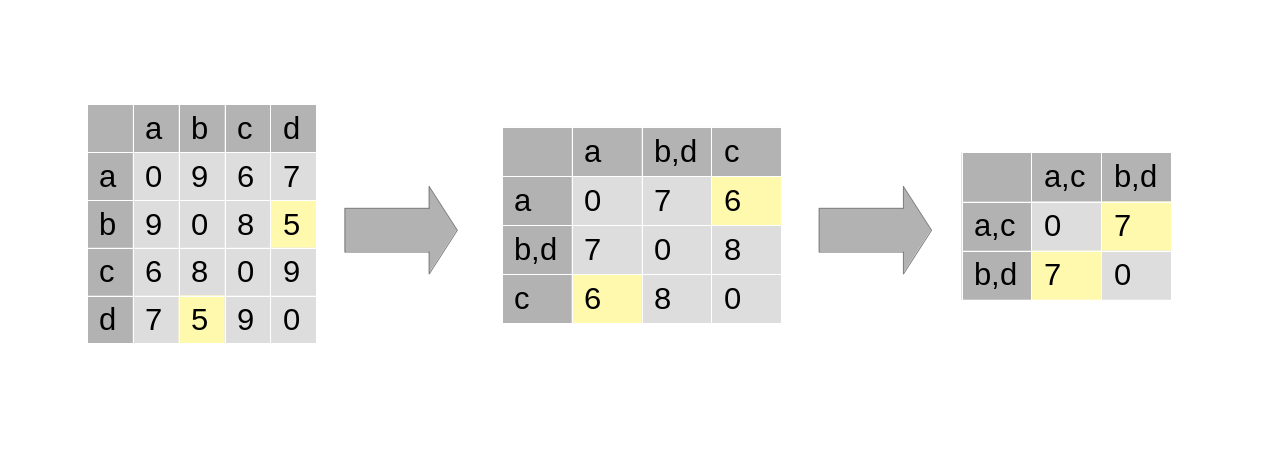
\includegraphics[width=\textwidth]{single_linkage}                                     
    \caption{Each table represents a distance matrix between pairs of nodes. In the first table, $d_{bd}$ marked in yellow is the shortest distance and therefore chosen to be part of the same cluster. The new node, or cluster, $(b,d)$ contain the shortest distances to the other nodes. In the second table, $d_{ac}$ is shortest and therefore put together in a cluster.}
    \label{fig:hierarch}
\end{figure}

\cref{fig:hierarch} illustrates how the algorithm works. 
In each iteration we choose the pair of nodes, or locations, with the smallest distance, $d_{ij}$ to be a part of a new cluster. The new distance matrix contain the shortest distance from the merged nodes to any other node. The merging of nodes goes on until we reach $k$ amount of nodes.

\subsubsection{Removing and inserting elements based on clusters}
In the previous sections we described how we can compare clusters of different sizes $k$, and how to find the best cluster for a given size. We used this in our model by running a preprocessiong algorithm that found the best clusters for different sizes of $k$. And then compared those clusters using the siluette coefficient to find the best possible cluster for a given distance matrix. \par

\begin{algorithm}
    \caption{Cluster heuristic}\label{alg:cluster}
    \begin{algorithmic}[1]
        \Function{cluster}{$s\in \{solution}$, $p$}
        \State select the number of orders to reinsert $q$
        \State add orders to array A acending based on cluster value $c_i$
        \State empty order set $I$
        \Repeat
            \State choose a random number $y$ between $[0,1]$
            \State remove the order in position $y^p$ in $A$ from $s$ 
            \State add removed order to $I$
        \Until {$|I| = q$}
        \For{$i\in I$}
            \State find vehicle schedule $S_v$ which maximizes $c_i$
            \State insert $i$ in best possible position in $S_v$
            \State update $s$ based on $S_v$
        \EndFor
        \State
        \Return $s$
        \EndFunction
    \end{algorithmic}
\end{algorithm}

\Cref{alg:cluster} start by selecting the amount of orders to remove. Then it sorts all orders from the given solution $s$ according to the cluster value $c_i$. $c_i$ is calculated based on the locations visited by the vehicle, ie. which other orders are bundled together on a schedule
We can define $c_i$ as:
\begin{equation}
    c_i = \dfrac{|L^P_{iv}|+|L^D_{iv}|}{|S_v|-2}
\end{equation}

Here the set $L^P_{iv}$ is locations from the same cluster $Cl^P_i$ as the pickup location $P$ of $i$ on vehicle $v$. 
$L^D_{iv}$ is a set of locations from the same cluster $Cl^D_i$ as the delivery location of $i$ on vehicle $v$. 
The set $S_v$ is the size of the schedule for vehicle $v$, ie. amount of locations visited. \par

To help explain how the $c_i$ works we give an example:
\begin{itemize}
    \item Vehicle 1 is transporting order 1, 2, and 3.
    \item Order 1 has a pickup location in cluster A and delivery location in cluster B.
    \item Order 2 has a pickup location in cluster B and delivery location in cluster C.
    \item Order 3 has a pickup location in cluster C and delivery location in cluster B.
\end{itemize}

For each location order 1 has in common with the other orders he is rewarded 1 point. Order 1's pickup location is unique. but the delivery location he shares with the pickup location of order 2 and delivery location of order 3. He is rewarded 2 points. \par
With this logic, order 2 is rewarded 3 points and order 3 is rewarded 3 points aswell.
To be able to compare these points with orders on other vehicles we divide the points on the maximum possible which is equal to $|S_v|-2$, or in the example $6-2 = 4$. 
The order with the smallest rank is order 1 with $\dfrac{2}{4}$. In other words two out of four locations visited, apart from the orders locations, belong to the same cluster as the pickup or delivery of order 1.
Order 2 and 3 have equally highest rank of $\dfrac{3}{4}$, ie. three out of four other locations belong to the same cluster as the pickup or delivery location of these orders. \par

In continuation of our \cref{alg:cluster} it uses the cluster ranking $c_i$ first to decide which orders to remove.
It will remove the orders with the lowest ranking, using some randomization, based on the value $p$. 
We choose to remove the order on the position $y^p$ in the $c_i$ sorted list of orders, where $y$ is a random number between $[0,1]$. We have chosen $p=4$ for all our heursitics.  \newline \par
To reinsert the orders we have chosen to try and insert the order by maximizing $c_i$. This means we find the vehicle schedule where the $c_i$ rank is the highest, and insert the order in the best possible position in the chosen vehicle. 

\subsection{Greedy}
\label{sec:greedy}
Removing orders in the most costful positions and reinserting it in its cheapest (greedy) position seems to be a reasonable way of moving towards a better solution.
We therefore propose a heuristic that removes the orders with the highest cost $c_{i}$.
The $c_i$ is calclated as the increase in a vehicles schedule cost with the chosen order.

\begin{algorithm}
    \caption{Greedy heuristic}\label{alg:greedy}
    \begin{algorithmic}[1]
        \Function{greedy}{$s\in \{solution}$, $p$}
        \State select the number of orders to reinsert $q$
        \State add orders in array $A$ based on decending cost $f(S_v) - f_{-i}(S_v)$
        \State empty order set $I$
        \Repeat
            \State choose a random number $y$ between $[0,1]$
            \State remove the order in position $y^p$ in $A$ from $s$ 
            \State add removed order to $I$
        \Until {$|I| = q$}
        \Repeat
            \State sort $I$ based on each orders minimum increase in objective value $c_i$
            \State insert the first order $i$ from $I$ in its best possible position in $s$
            \State remove order $i$ from $I$
        \Until{$|I| = 0$}
        \State
        \Return $s$
        \EndFunction
    \end{algorithmic}
\end{algorithm}

We remove orders again based on the same randomness factor explained above. 
We do this by first sorting the orders decending based on $c_i$. $c_i$ can be calculated as $c_i=f(S_v) - f_{-i}(S_v)$. 
Here the $-i$ indicate that the vehicle schedule $S_v$ is without the order $i$.
We then choose the order in the $y^p$ position. \par

To reinsert an order we simply sort the removed orders based on their $c_i$.
The $c_i = \min(\Delta f_{iv})$, were the $\Delta f_{iv}$ is the lowest increase in objective function value when inserting $i$ in a vehicle schedule $v$. The $c_i$ is therefore the minimum of theseincreases. 
We reinsert the order in its best possible position in vehicle schedule $v$ and update the solution $s$. 

\subsection{Similar regret}
\label{sec:shaw}
The removal part of this heuristic is based on \citet{shaw97}'s removal heuristic with slight modifications based on our problem. 
It removes orders that share specific similar qualities. 
The basic idea is that replacing these orders by eachother will find new, hopefully better, solutions. 
We define a relatedness factor $r_{ij}$ which represents how much the order $i$ is related to the order $j$. 
The lower the value of $r_{ij}$ the more the two orders $i$ and $j$ are related.
The relatedness of two orders were based on the following properties: 
a distance property, a weight property, an overlapping timewindow property, a property indicating if the same vehicles can be used to serve each request, and finally if the orders belong to the same factory.

The relatedness factor is given by the following equation:

\begin{equation}
\label{relatedness}
    r_{ij} = \psi ( D_{i j} + D_{(i+n)(j+n)}) + \omega|Q_i - Q_j|
    + \phi (1-\dfrac{|V_i\cap V_j|}{max(|V_i|, |V_j|)} ) + \tau G_{ij} + \chi (U_{ij} + U_{(i+n)(j+n)})
\end{equation}
Thus the relatedness measure $r_{ij}$ is given a value $0\leq r_{ij} \leq 2\psi + \omega + \phi + \tau  + \chi$. 
We have chosen the following values in this paper $\psi=0.7$, $\omega=1.0$, $\phi=0.8$, $\tau=0.3$, $\chi = 0.3$. \par

$D_{ij}$, $Q_i$, are the same as in \cref{ch:mm} and all values have been normalised to result in a value between $[0..1]$. 
$V_i$ is the set of vehicles that can serve order $i$. 
The parameter $G_{ij}$ is 1 if $i$ belong to another factory than $j$ and 0 if they belong to the same factory. 
$U_{ij}$ is the timewindows at the pickup and delivery location, equal to 0 if the two orders have identical time windows and 1 if not. It corresponds to the sum of overlapping time windows divided by the overlapping span of the two time window sets.
It can be formulated as follows:
\begin{equation}
    \label{overlaptime}
    U_{ij} = 1 - 
    \dfrac{T^O_{ij}}
    {\max{(\max\limits_{p\in \pi_i} \overline{T_{ip}}, \max\limits_{o\in \pi_j} \overline{T_{jo}})} - 
    \min{(\min\limits_{p\in \pi_i} \underline{T_{ip}}, \min\limits_{o\in \pi_j} \underline{T_{jo}}}) -  T^{NO}_{ij} }
\end{equation}

Here $\overline{T_{ip}}$ and $\underline{T_{ip}}$ are the upper and lower time windows defined in the problem formulation.
The factor $T^O_{ij}$ consists of all the timewindows where order $i$ overlaps with the timewindows from order $j$. It can be written mathematically as follows:
\begin{equation}\label{eq:ot}
    T^O_{ij}=\sum\limits_{\substack{p\in \pi_i\\ o\in \pi_j\\ \underline{T_{ip}}\leq \overline{T_{jo}}\\ \underline{T_{jo}}\leq\overline{T_{ip}}}} (\min(\overline{T_{ip}}, \overline{T_{jo}}) - \max(\underline{T_{ip}},\underline{T_{jo}}) )
\end{equation}

The factor $T^{NO}_{ij}$ is the opposite of the above factor $T^O_{ij}$ and represent the time when neither $i$ not $j$ have a timewindow. This can be examplified by night time when no factory is open. It can be formulated as follow:

\begin{equation}\label{eq:not}
    T^{NO}_{ij} = \sum\limits_{\substack{p\in \pi_i\\ o\in \pi:q_j\\ \underline{T_{ip}}\geq \overline{T_{j(o-1)}}\\ \underline{T_{jo}}\geq\overline{T_{i(p-1)}}}} 
    (\min(\underline{T_{ip}}, \underline{T_{jo}}) - \max(\overline{T_{i(p-1)}},\overline{T_{j(o-1)}}) ) 
\end{equation}

\begin{algorithm}
    \caption{Similar regret heuristic}\label{alg:simReg}
    \begin{algorithmic}[1]
        \Function{similarRegret}{$s\in \{solution}$, $p$}
        \State select the number of orders to reinsert $q$
        \State select a random order $i$ from $s$
        \State add $i$ to order set $I$
        \Repeat
            \State add all orders $j\not\in I$ in array $A$ acending based on relatedness $r_{ij}$
            \State choose a random number $y$ between $[0,1]$
            \State remove the order in position $y^p$ in $A$ from $s$ 
            \State add removed order to $I$
        \Until {$|I| = q$}
        \Repeat
            \State sort $I$ acending based on regret value $c^*_i$
            \State insert the first order $z$ from $I$ in its best possible position in $S_v$
            \State update $s$ based on $S_v$
            \State remove order $z$ from $I$
        \Until{$|I| = 0$}
        \State
        \Return $s$
        \EndFunction
    \end{algorithmic}
\end{algorithm}


\Cref{alg:simReg} is s pseudocode of the complete similar regret heursitic.
It starts by removing a random order $i$ from the solution and adding it to a set $I$. 
It then creates an array and adds all orders $j\not\in I$ to this array, before it sorts it acending based on $r_{ij}$.
It then selects the order with the $y^p$ highest relatedness to remove from $s$ and add to $I$. This continues until $q$ orders have been removed.
The insertion part of this heuristic tries to improve on insertion algorithm from \cref{sec:greedy} by calculating a regret value, $c^*_i$. The regret value tries to predict the "what if i insert later" value of an order $i$. 
If we let $v_{ik} \in \{ 1,..,m\}$ represent a vehicle schedule for which $i$ has the $k$ lowest insertion cost. 
That means $\Delta f_{s_{ik}} \leq \Delta f_{s_{ik'}}$ for $k\leq k'$.
We can then define the regret value as follows:
\begin{equation}\label{eq:regret}
    \centering
    c^*_i=\Delta f_{v_{i2}} - \Delta f_{v_{i1}} + \Delta f_{v_{i3}} - \Delta f{v_{i2}}
\end{equation}

The $c_i$ therefore represent the difference in inserting order $i$ in its best position and its second best position plus the difference in inserting it in its second best position and its third best position. In each iteration the heuristic chooses to insert the order with the highest $c^*_i$. The order will be inserted in its best possible position. Ties were broken by choosing the order with the lowest $c_i$.

\section{Choosing a heuristic}
\label{sec:choosing}
We proposed several heuristics of different classes in the previous sections, and one could simply choose one of them and use them throughout the search. 
However we propose to use all the heuristics, for now. 
The reason for doing so is that the swap heuristic from \cref{sec:swap} could be good for one type of instance, while the similar regret heuristic from \cref{sec:exch} might be good for another type of instance. 
We think that alternating between several type of heuristics gives us amore robust algorithm. 
We will however do alot of testing in \cref{ch:res}, which will lead us to a more compact version of the model. \par
To select a heuristic to use in each iteration of \cref{alg:alns}, we have used the \emph{roulette weel principle} from \cite{hemmati14}. 
This means that is we represent each heuristic by a number $i \in [1..m]$ where m is the amount of heuristics. 
We select a heuristic with a probability $p_i$ calculated based on each heuristics \textit{weight} $w_i$ as follows:
\begin{equation}\label{eq:weights}
    p_i=\dfrac{w_i}{\sum_{j=1}^m w_j}
\end{equation}

Notice we are using one probability per heuristic and not per insertion and removal heuristic like \cite{ropke06}. These weights could be set fixed per problem but we choose to use an adaptive weight system explained futher in \cref{sec:weight}.

\section{Adaptive weight adjustment}
\label{sec:weight}
The weights from \cref{sec:choosing} can be adapted automatically by the algorithm. 
The basic idea is to keep track of the perfomance of each heuristic through a scoring system. 
A heuristic is given a higher score for a better performance and a low score for low performance. 
The entire \cref{alg:alns} is divided into \textit{segments}, or a numer of iterations. 
We have used segments here of 100 iterations.
At the beginning of the algorithm, each heuristic is given the same weights, resulting in equal probability in selecting each heuristic for the first segment.
Throughout a segment, each heuristic is rewarded points based on the following system:
\begin{itemize}
    \item Finding a new global best solution is given a high score to the heuristic for that iteration.
    \item Finding a new solution that is better than the current solution gives a medium score to the heuristic for that iteration.
    \item Finding a new solution that has not been found before is rewarded a small score to the heuristic for that iteration.
\end{itemize}
After a segment, the sum of the scores for each heuristic are used to update the weights. If we let $w_{ij}$ be the weight of heuristic $i$ in segment $j$ the update would be as follows:
\begin{equation}\label{eq:update}
    w_{ij} = w_{i(j-1)}h + (1-h)\dfrac{\pi_i}{\lambda_i}
\end{equation}

The $h$ represent here a historical weight factor which we have set to $80\%$ meaning we let the previous weight compose $80\%$ of the new weight. 
$20\%$ of the current weight $w_{ij}$ is composed of the score $\pi_i$ divided over the times we have run the heuristic $\lambda_i$ during the current segment.

\begin{figure}                                                                    
    \centering                                                                                     
    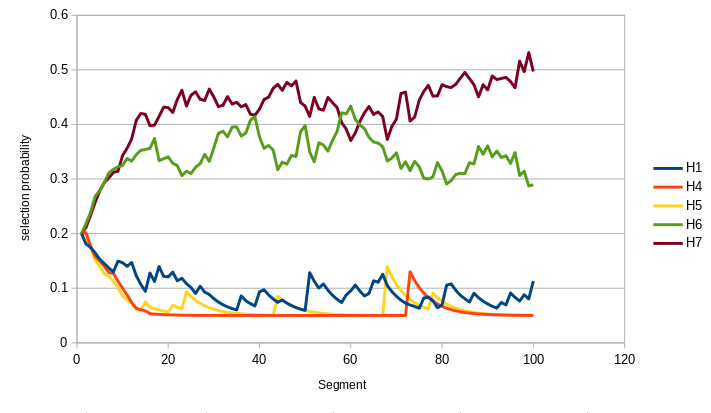
\includegraphics[width=.7\textwidth]{weight_probability}                                     
    \caption{The figure illustrates an example of the developement of the weight probability $p_i$ when running our model. The x-axis represent a segment and the y-axis the probability of selecting a heuristic.}
    \label{fig:weights}
\end{figure}

\Cref{fig:weights} show how the weight probability $p_i$ developes for five different heuristics in an example from our model. 
We observe that the probability start out equal but that some heuristics are getting more probability after only a few segments.
The figure also shows that we have put a lower limit to the probility to make certain that every heuristic will be selected at least a few times during a segment.

\section{Acceptance criteria and stopping condition}
\label{sec:accept}
We could only accept solutions that are better than the current one.
However this could lead our model to get stuck in a local neighbourhood and not be able to get out of it. 
We have therefore chosen to use the acceptance criteria used by simmulated annealing, mentioned in \cref{ch:solMeth}. 
This acceptance criteria is made so that it accepts a solution that is better than the current solution. It also accepts a worse solution with the probability $e^{-|f-f_{new}|/T}$, where $T<0$ is the temperature. 
The cooling schedule we use here was implemented by \cite{crama03}. That sets a certain starting temperature $T_{start}$ that decreases per iteration with a certain cooling rate $0<c<1$.
We wanted to let $T_{start}$ depend on the problem instance our model is trying to solve. Therefore we run 100 iterations with a fixed acceptance rate of $a = 0.8$. 
We calculate the average of all worse solutions that are accepted over these iterations $f^T_{average}$.  
Then we use this to calculate the fitting starting temperature as follows:
\begin{equation}\label{eq:startTemp}
    T_{start} = \dfrac{f^T_{average}}{log(a)}
\end{equation}

The algorithm stops when a specified number of iterations are reached which we specify here as 10 thousand iterations per run.

\section{Wild escape algorithm}
\label{sec:wild}
Algorithms containing large neighbourhood heuristics, such as our model, are known to be good at searching locally aswell as globally. 
However they do sometimes get stuck in one neighbourhood, and it is important that our algorithm is able to react in these situations.
We designed an algorithm as part of our model that reacts if a certain criteria is fulfilled. \Cref{alg:alns} shows that if a certain criteria is fulfilled we will run an escape algorithm.
We set the criteria that if for 500 iterations we do not find an improvement in $s_{best}$ we will run the algorithm we call escape algorithm. 

\begin{algorithm}
    \label{alg:wild}
    \caption{Wild escape algorithm}
    \begin{algorithmic}[1]
        \Function{wildEscape}{$s\in solution,s_{best}$, set of heuristics $H$}
        \Repeat
            \State choose a random heuristic $h$ from $H$
            \State apply $h$ to $s$
            \If {$f(s)<f(s_{best})$}
                \State $s_{best} = s$
            \EndIf
        \Until stop condition met
        \State \Return $s$
        \EndFunction
    \end{algorithmic}
\end{algorithm}

The algorithms pseudocode is described in \cref{alg:wild}. The stopping criteria of the algorithm is 20 iterations. 
The algorithm accepts any new solution found regardless of the objective value.
The heuristics used by the escape algorithm are the heuristics random fit from \cref{sec:rand}, 3-exchange from \cref{sec:exch} and swap \cref{sec:swap}. The heuristics have an increased size of $q$so that they can move further away from the current neighbourhood. We chose these heuristics because they are not trying to improve the solution in any specific way and select targeted solutions, but rather moves randomly around the solution space. 
\biblio                                                         
\end{document}
